\documentclass[tikz,border=5]{standalone}
\usepackage{tikz}
\usetikzlibrary{shapes.geometric, arrows, positioning, fit, calc}



\begin{document}
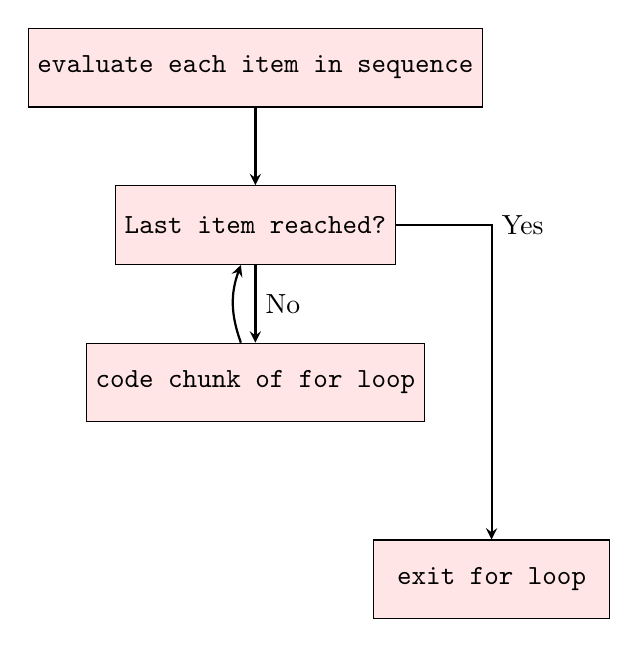
\begin{tikzpicture}
	
	\tikzstyle{chunk} = [rectangle, minimum width=3cm, minimum height=1cm, text centered, draw=black, fill=red!10]
	\tikzstyle{arrow} = [thick,->,>=stealth]
	
	\node (evaluation) [chunk] at (12,4.5) {\texttt{evaluate each item in sequence}};
	\node (last) [chunk] at (12,2.5) {\texttt{Last item reached?}};
	\node (code) [chunk] at (12,0.5) {\texttt{code chunk of for loop}};
	\node (exit) [chunk] at (15,-2) {\texttt{exit for loop}};
	
	\draw [arrow] (evaluation) -- (last);
	\draw [arrow] (last) -| node[right] {Yes} (exit);
    \draw[arrow] (last) -- node[right] {No} (code);
    \draw[arrow] (code) to[bend left=20]  (last);
 
\end{tikzpicture}
\end{document}